%
% 
%
% Copyright (C) 1997-2013 by Dimitri van Heesch.
%
% Permission to use, copy, modify, and distribute this software and its
% documentation under the terms of the GNU General Public License is hereby 
% granted. No representations are made about the suitability of this software 
% for any purpose. It is provided "as is" without express or implied warranty.
% See the GNU General Public License for more details.
%
% Documents produced by Doxygen are derivative works derived from the
% input used in their production; they are not affected by this license.

\documentclass{book}
\usepackage[a4paper,left=2.5cm,right=2.5cm,top=2.5cm,bottom=2.5cm]{geometry}
\usepackage{makeidx}
\usepackage{natbib}
\usepackage{graphicx}
\usepackage{multicol}
\usepackage{float}
\usepackage{geometry}
\usepackage{listings}
\usepackage{color}
\usepackage{ifthen}
\usepackage[table]{xcolor}
\usepackage{textcomp}
\usepackage{alltt}
\usepackage{ifpdf}
\ifpdf
\usepackage[pdftex,
            pagebackref=true,
            colorlinks=true,
            linkcolor=blue,
            unicode
           ]{hyperref}
\else
\usepackage[ps2pdf,
            pagebackref=true,
            colorlinks=true,
            linkcolor=blue,
            unicode
           ]{hyperref}
\usepackage{pspicture}
\fi
\usepackage[utf8]{inputenc}
\usepackage{mathptmx}
\usepackage[scaled=.90]{helvet}
\usepackage{courier}
\usepackage{sectsty}
\usepackage[titles]{tocloft}
\usepackage{amssymb}
\usepackage{doxygen}
\lstset{language=C++,inputencoding=utf8,basicstyle=\footnotesize,breaklines=true,breakatwhitespace=true,tabsize=8,numbers=left }
\makeindex
\setcounter{tocdepth}{3}
\renewcommand{\footrulewidth}{0.4pt}
\renewcommand{\familydefault}{\sfdefault}
\renewcommand{\cftsecindent}{0 em}
\renewcommand{\cftsecnumwidth}{3.2 em}
\renewcommand{\cftsubsecindent}{3.2 em}
\newcommand{\thisyear}{\the\year}
\hfuzz=15pt
\setlength{\emergencystretch}{15pt}
\hbadness=750
\tolerance=750
\begin{document}
\begin{titlepage}
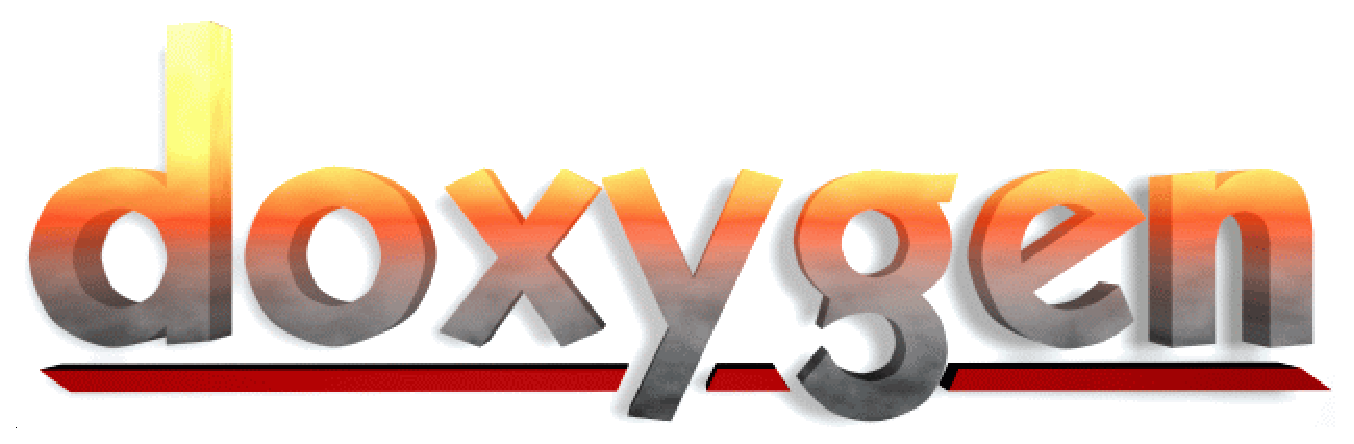
\includegraphics[width=\textwidth]{doxygen_logo}
\begin{center}
Manual for version $VERSION\\[2ex]
Written by Dimitri van Heesch\\[2ex]
\copyright 1997-\thisyear
\end{center}
\end{titlepage}
\clearemptydoublepage
\tableofcontents
\clearemptydoublepage
\pagenumbering{arabic}
\begin{DoxyVerb}Contents:
- @ref fdhwlib_intro
- @ref fdhwlib_usage
- @ref fdhwlib_dirs
- @ref fdhwlib_build
- @ref fdhwlib_version
\end{DoxyVerb}
\hypertarget{index_fdhwlib_intro}{}\section{Introduction}\label{index_fdhwlib_intro}
This document contains a description of the hardware access library for the Pierre Auger Fluoresence Detector Electronic (F\-E) other experiments. The library provides (nearly) the same functionality for Linux and Windows and Apple operating system.

The library is divided in three layers\-:
\begin{DoxyItemize}
\item api This layer provides the interface to the for the application programms. The function of this layer are rather independent from the realization of the hardware.
\item The register model layer implements the address model of the hardware. Changes in the hardware structure will also cause changes in this layer. This means also that for the different experiments own register models exist. Implemented are\-:
\begin{DoxyItemize}
\item basehw
\item hw
\item katrinhw
\end{DoxyItemize}
\item pbus This layer provides the interface to the hardware via the Pbus protocol (simple V\-M\-E bus type).
\end{DoxyItemize}

Included in the package are some more general utility functions\-:
\begin{DoxyItemize}
\item \hyperlink{group__akutil__group}{Utility functions + classes}
\begin{DoxyItemize}
\item \hyperlink{timesync}{Relation between P\-C clock and G\-P\-S time}
\end{DoxyItemize}
\item simpleshell
\item calib\-\_\-group
\item ts\-\_\-group
\begin{DoxyItemize}
\item bgformat
\item fddaswin
\end{DoxyItemize}
\item \hyperlink{classgps}{gps}
\begin{DoxyItemize}
\item gps\-\_\-remote
\item gps\-\_\-conf
\end{DoxyItemize}
\end{DoxyItemize}

\begin{DoxyVerb}Dependancies of the libraries in the package
\end{DoxyVerb}


\begin{DoxyVerb}   akutil
  
   akshell -- akutil
  
   
   calib -- Hw -- Pbus\<AccessType\> -- akutil
  
   am_testutil -- Hw -- Pbus\<AccessType\> -- akutil
  
   FEdata --Hw --Pbus\<AccessType\> -- akutil
    
  
   FE -- Hw -- Pbus\<AccessType\> -- akutil
  
   Hw -- Pbus\<AccessType\> -- akutil
   
   Pbus\<AccessType\> -- akutil \end{DoxyVerb}
\hypertarget{index_fdhwlib_usage}{}\section{Usage}\label{index_fdhwlib_usage}
Projects using the hardware access library need to add the directory fdhwlib/fdhwlib to their include path.

Example (Auger A\-P\-I)\-: \begin{DoxyVerb}#include <FE/FE.h>

main(){

  FE fe;
  FE fe.config.init();
  ...

}
\end{DoxyVerb}
 Linking the project it is necessary to add the hardware access library and Pbus library.

Example (Katrin Register Model)\-: \begin{DoxyVerb}#include <katrinhw/kasubrack.h>

main(){

   KaSubrack *s;
   s = new KaSubrack(katrin.ini);
   ...
}  
\end{DoxyVerb}
\hypertarget{index_fdhwlib_dirs}{}\section{Directory Structure}\label{index_fdhwlib_dirs}
The directory fdhwlib contains project file for Kdevelop/\-Linux and M\-S Visual C++/\-M\-S Windows to create the approritate version of the library. The sources for the different layers can be found in the directories fdhwlib/F\-E, fdhwlib/\-Hw and fdhwlib/Pbus. Some more general utilities will be found in fdhwlib/akutil. The definition of the K\-A\-T\-R\-I\-N hardware model is based on the same generic classes used in the Auger register model. All K\-A\-T\-R\-I\-N specific classes can be found in fdhwlib/katrinhw

The documentation generated can be found in the directory fdhwlib-\/api. It is available in html and latex format.\hypertarget{index_fdhwlib_build}{}\section{Compilation of the libraries}\label{index_fdhwlib_build}
\hypertarget{index_buildlinux}{}\subsection{Linux}\label{index_buildlinux}
To compile and install the library use the commands \begin{DoxyVerb}./configure
./makeAll
./makeAll daq
./make doc
./makeInstall
./makeInstall daq
\end{DoxyVerb}
 Without the argument \char`\"{}daq\char`\"{} no fd-\/das or R\-O\-O\-T support is required. For most applications it may be sufficient to omit creating the fd-\/daq dependant part of the package.

The package requires some external packages. These are Root, fd-\/das and the micro\-Enable drivers. Use the environment variable C\-P\-L\-U\-S\-\_\-\-I\-N\-C\-L\-U\-D\-E\-\_\-\-P\-A\-T\-H to specify the path to the header files. E.\-g. use \begin{DoxyVerb}CPLUS_INCLUDE_PATH=/usr/software/fdhwlib/include:
       /home/kopmann/FD-das/include:/home/kopmann/FD-das/mirror/include:
       /cern/root/include:/usr/src/menable/include:/usr/lib/qwt/include:
\end{DoxyVerb}
 \begin{DoxyVerb}To install the package it is necessary to have write
access to the install directory /usr/software.
\end{DoxyVerb}
\hypertarget{index_buildwindows}{}\subsection{Windows}\label{index_buildwindows}
For all libraries a M\-S\-V\-C project exists. Use these to compile a separate library.

To generate all libraries use the script fdhwlib/make\-All.\-bat. The script accepts two additional arguments to generate the menable and daq dependant parts of the library. For these libraies it is required to specify the location of the required packages (menable + daq + root) in the I\-N\-C\-L\-U\-D\-E environment variable. The path of the root libraries has to be added to to the L\-I\-B environment variable.

\begin{DoxyVerb}makeAll                  Generate the standard libraries
makeAll menable          Generate menable depandant part
makeAll daq              Generate daq dependant part
\end{DoxyVerb}
 \begin{DoxyVerb}To use the libraries add the directory fdhwlib/fdhwlib to the include
path and all required fdhwlib/fdhwlib/\<subdir\>/debug directories
(e.g. fdhwlib/fdhwlib/Hw/debug) to the library path.
\end{DoxyVerb}
\hypertarget{index_builddoc}{}\subsection{Documentation}\label{index_builddoc}
The documentation can be automatically generated from the header files using doxygen (or other programs handling javadoc type comments).

Using \char`\"{}make doc\char`\"{} will generate documentation for all packages.\hypertarget{index_buildinternals}{}\subsection{Build system internals}\label{index_buildinternals}
The packages uses the standard build system of the kdevelp I\-D\-E and M\-S\-V\-C where this is possible and sufficient. However in some case it turned out to be adequate to provide additional scripts. The scripts are named on both platforms as \char`\"{}make\-All\char`\"{} and \char`\"{}make\-Install\char`\"{}. The scripts will accept additional arguments (\char`\"{}daq\char`\"{}, \char`\"{}meanble\char`\"{}) to create microenable or D\-A\-Q dependant parts of the package.

Central with kdevelop are the files Makefile.\-am in every directory of the projects. The configure step will generate from this file the required Makefiles. Some manual work has to be done in the scripts to activate all make options and to install some parts that are not installed automatically.

In M\-S\-V\-C the information of the build process is hidden in the D\-S\-P project files. It is possble to generate makefiles (extension M\-A\-K) for Microsofts nmake program. The redundand M\-A\-K files allow to build the whole project automatically from the command line and to control the make process by script files.\hypertarget{index_fdhwlib_version}{}\section{Remark on version numbers}\label{index_fdhwlib_version}
\begin{DoxyVerb}There are several version numbers used in the package
fdhwlib. First comes the overall version of the package
It can be found in the files fdhwlib.h config.h (only in the
development version, not included in the tar-ball!) somewhere
in the kdevelop project file and in the doxygen configuration.
The project file will automatically update config.h but not
the other places. This has to be done manually. All files
should show the same version number.

There are other version numbers that are hardware related.
The purpose of these numbers is to keep the library compatible
with older versions of the hardware design. The version numbers
are used in this case for conditional comiplation.
(PBUS_VER, FLT_VER and FLT_VER).\end{DoxyVerb}
 
\part{User Manual}
\chapter{Installation}\label{install}\hypertarget{install}{}\input{install}
\chapter{Getting Started}\label{starting}\hypertarget{starting}{}\input{starting}
\chapter{Documenting the code}\label{docblocks}\hypertarget{docblocks}{}\input{docblocks}
\chapter{Markdown}\label{markdown}\hypertarget{markdown}{}\input{markdown}
\chapter{Lists}\label{lists}\hypertarget{lists}{}\input{lists}
\chapter{Grouping}\label{grouping}\hypertarget{grouping}{}\input{grouping}
\chapter{Including Formulas}\label{formulas}\hypertarget{formulas}{}\input{formulas}
\chapter{Graphs and diagrams}\label{diagrams}\hypertarget{diagrams}{}PROJECT_NAME       = "Diagrams"
OUTPUT_DIRECTORY   = diagrams
HAVE_DOT           = YES
EXTRACT_ALL        = YES
GENERATE_LATEX     = NO
GENERATE_MAN       = NO
GENERATE_RTF       = NO
CASE_SENSE_NAMES = NO
ENABLE_PREPROCESSING       = YES
INPUT              = .
FILE_PATTERNS      = diagrams_*.h
QUIET              = YES
JAVADOC_AUTOBRIEF = YES
SEARCHENGINE     = NO

\chapter{Preprocessing}\label{preprocessing}\hypertarget{preprocessing}{}\input{preprocessing}
\chapter{Automatic link generation}\label{autolink}\hypertarget{autolink}{}PROJECT_NAME     = "Automatic link generation"
OUTPUT_DIRECTORY = autolink
GENERATE_LATEX   = NO
GENERATE_MAN     = NO
GENERATE_RTF     = NO
CASE_SENSE_NAMES = NO
INPUT            = autolink.cpp
QUIET            = YES
JAVADOC_AUTOBRIEF = YES
SEARCHENGINE     = NO

\chapter{Output Formats}\label{output}\hypertarget{output}{}\input{output}
\chapter{Searching}\label{searching}\hypertarget{searching}{}\input{searching}
\chapter{Customizing the Output}\label{customize}\hypertarget{customize}{}\input{customize}
\chapter{Custom Commands}\label{custcmd}\hypertarget{custcmd}{}\input{custcmd}
\chapter{Link to external documentation}\label{external}\hypertarget{external}{}\input{external}
\chapter{Frequently Asked Questions}\label{faq}\hypertarget{faq}{}\input{faq}
\chapter{Troubleshooting}\label{trouble}\hypertarget{trouble}{}\input{trouble}
\part{Reference Manual}
\chapter{Features}\label{features}\hypertarget{features}{}\input{features}
\chapter{Doxygen usage}\label{doxygen_usage}\hypertarget{doxygen_usage}{}\input{doxygen_usage}
\chapter{Doxywizard usage}\label{doxywizard_usage}\hypertarget{doxywizard_usage}{}\input{doxywizard_usage}
\chapter{Configuration}\label{config}\hypertarget{config}{}\input{config}
\chapter{Special Commands}\label{commands}\hypertarget{commands}{}\input{commands}
\chapter{HTML commands}\label{htmlcmds}\hypertarget{htmlcmds}{}\input{htmlcmds}
\chapter{XML commands}\label{xmlcmds}\hypertarget{xmlcmds}{}\input{xmlcmds}
\part{Developers Manual}
\chapter{Doxygen's internals}\label{arch}\hypertarget{arch}{}\input{arch}
\chapter{Perl Module Output format}\label{perlmod}\hypertarget{perlmod}{}\input{perlmod}
\chapter{Internationalization}\label{langhowto}\hypertarget{langhowto}{}\input{langhowto}
\printindex
\end{document}
